\documentclass[letterpaper]{article} % DO NOT CHANGE THIS
\usepackage[submission]{aaai2027}  % DO NOT CHANGE THIS
\usepackage[hyphens]{url}  % DO NOT CHANGE THIS
\usepackage{graphicx} % DO NOT CHANGE THIS
\urlstyle{rm} % DO NOT CHANGE THIS
\def\UrlFont{\rm}  % DO NOT CHANGE THIS
\usepackage{natbib}  % DO NOT CHANGE THIS AND DO NOT ADD ANY OPTIONS TO IT
\usepackage{caption} % DO NOT CHANGE THIS AND DO NOT ADD ANY OPTIONS TO IT
\frenchspacing  % DO NOT CHANGE THIS
\setlength{\pdfpagewidth}{8.5in} % DO NOT CHANGE THIS
\setlength{\pdfpageheight}{11in} % DO NOT CHANGE THIS
\usepackage{amsmath,amssymb,amsthm}
\usepackage{booktabs}
\usepackage{xcolor}
\pdfinfo{
/TemplateVersion (2027.1)
}
\setcounter{secnumdepth}{0}

\newtheorem{proposition}{Proposition}
\newcommand{\Ltriv}{L_{\mathrm{triv}}}
\newcommand{\kstar}{k^\star}

\title{Pruning Attention Heads the Way the Brain Prunes Vessels}
\author{Anonymous Submission}
\affiliations{}

\begin{document}
\maketitle

\begin{abstract}
Transformers keep more attention heads than their tasks need, and pruning methods decide how many to keep by hand. The brain sizes its blood supply without a target: vessels that carry little flow regress, and Murray's law sets vessel size by trading the work of pumping blood against its upkeep. We propose \emph{hemodynamic attenuation}, a pruning rule built on this principle. Each attention head pays a fixed upkeep, is valued after the other heads compensate for it, and closes gradually when it is worth less than its upkeep. Because the rule minimizes a single cost, loss plus upkeep, what it keeps can be predicted before training, and one setting, an upkeep of 1\% of the loss the heads remove, worked on both the benchmark and GPT-2 without a target size. On a new task whose minimal number of heads is known, it kept exactly that number in 29 of 30 runs while the task stayed solved, which none of the published methods we tested achieved. Two further predictions of the cost held: the upkeep at which the rule collapses, and the number of backup heads kept under random head failure, matched exactly in 79 of 100 runs predicted in writing beforehand. When demand changed during training, the rule closed and reopened heads to follow it. Trained from scratch to copy repeated text, it kept the heads of the known induction circuit in 10 of 10 runs. On GPT-2 small, it recovered the core of the hand-mapped indirect-object circuit, stable across prompt samples: with 20--21 heads instead of 26, it matched the published circuit's accuracy and favored the correct name more strongly.
\end{abstract}

\begin{figure}[!t]
\centering
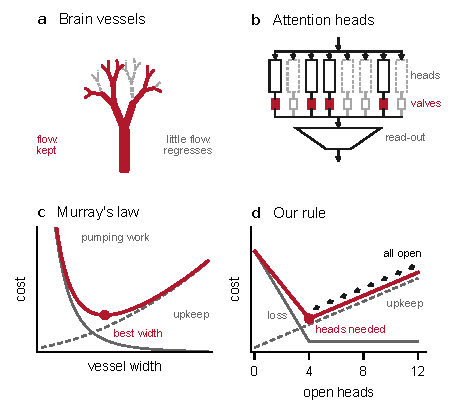
\includegraphics[width=\columnwidth]{fig_hero.pdf}
\caption{From vessels to heads (illustration). \textbf{(a)} Brain vessels that carry little flow regress (dashed), and the rest are kept. \textbf{(b)} Each attention head passes through a valve. Heads worth less than their upkeep are closed (gray). \textbf{(c)} Murray's law: a vessel's width minimizes the work of pumping blood plus the upkeep of the blood it holds. \textbf{(d)} Our rule: loss falls until the needed heads are open and upkeep grows with each one, so closing heads lowers the sum until only the needed heads remain. A design principle, not a model of blood flow.}
\label{fig:hero}
\end{figure}

\begin{figure*}[!t]
\centering
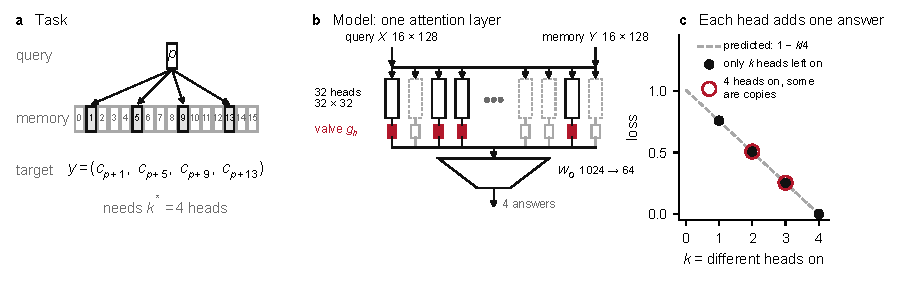
\includegraphics[width=\textwidth]{fig_task.pdf}

\vspace{2pt}
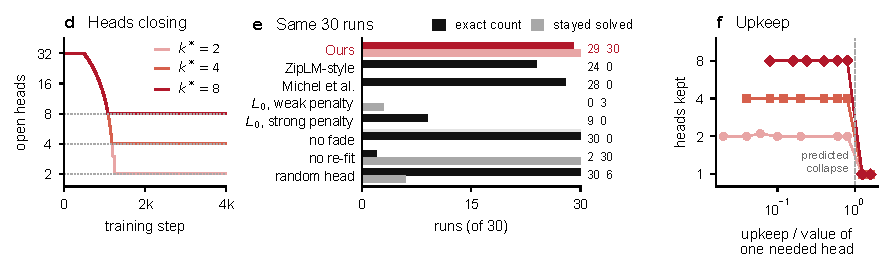
\includegraphics[width=\textwidth]{fig_neuroai_row.pdf}
\caption{A task with a known minimal circuit, and the results on it. \textbf{(a)} A query names a position $p$, and the target is the items at $R$ fixed offsets. Here $R=4$, so 4 heads are needed. \textbf{(b)} The model, with sizes. Each head has a valve $g_h$ (red when open) and pays an upkeep while open. \textbf{(c)} Loss of a trained model with only $k$ heads on (black) follows $1-k/R$ (dashed). With copies among the heads (red), only \emph{different} heads count: a copy is worth nothing. Units of $\Ltriv$. \textbf{(d)} Open heads during training, one run per task size, with $\kstar$ dotted. \textbf{(e)} Every method on the same 30 runs ($\kstar=2,4,8$, 10 seeds each), all run in our code \citep{ziplm,michel2019sixteen,voita2019analyzing}. ZipLM uses our score once, then fine-tunes. ZipLM and Michel et al.\ were given the true count. $L_0$ gates are shown at the weakest and strongest of three penalties ($\lambda=0.05$ and $1$). The lower three rows each remove one part of our rule. \textbf{(f)} Heads kept against the upkeep, in units of the value of one needed head, $\Ltriv/R$. Theory predicts $\kstar$ heads left of 1 and one head right of it (3 seeds per point).}
\label{fig:task}
\end{figure*}

\section{Introduction}

A trained transformer usually has more attention heads than its task needs \citep{michel2019sixteen,voita2019analyzing}, and trained models keep backup heads that take over when others are removed \citep{wang2023interpretability,mcgrath2023hydra}. Existing pruning methods fix the final size by hand, as a target sparsity \citep{zhu2017prune}, a penalty strength \citep{voita2019analyzing,nam2025chg} or a threshold \citep{conmy2023towards}, and most prune after training. None of them predicts the size it will reach or how much redundancy it will keep (Table~\ref{tab:related}). And benchmarks with known circuits build the circuit in by construction \citep{lindner2023tracr,gupta2024interpbench}, so they cannot test whether a method finds the minimal circuit among the redundant heads that training produces.

The cerebral circulation solves a similar allocation problem without a target size. The neurovascular unit senses local demand and adjusts vessel diameter \citep{iadecola2017nvu}. Vessels that carry little flow regress gradually rather than being cut \citep{korn2015pruning}, and tissue survives the loss of a vessel when collaterals supply its territory. Where demand returns, new vessels grow. \citet{murray1926} showed that vessel size follows from minimizing the work of moving blood plus the metabolic cost of keeping it. By the same logic, a vessel is worth keeping only while it earns its upkeep.

We carry this principle over to attention heads (Figure~\ref{fig:hero}). Every head has a valve and pays a fixed upkeep while the valve is open. A head is valued by the loss that would remain if it closed and the other heads adjusted to cover for it, the analog of collateral flow. A head worth less than its upkeep is closed gradually, and a closed head reopens if it becomes valuable. Nothing in the rule names a target size. Our contributions are:
\begin{itemize}
\item \emph{Hemodynamic attenuation}, a rule that charges each head a fixed upkeep, values it after the other heads compensate, and closes heads gradually during training. It minimizes loss plus upkeep (Proposition~1), so it makes predictions before training.
\item A shared benchmark for AI and neuroscience: its minimal circuit is known in size and roles, while the redundancy comes from training.
\item Three predictions of the objective confirmed: the head count, the upkeep at which the rule collapses, and the redundancy kept under failure.
\item Adaptation to changing demand, where reopening alone fails and a second vascular mechanism, sprouting, is needed.
\item Known circuits recovered: induction, and a stable core of the indirect-object circuit in GPT-2 small that matches the published circuit with fewer heads. Heads hidden by their backups are found by re-valuing and missed by ranking once.
\end{itemize}

\begin{table}[t]
\centering
\footnotesize
\setlength{\tabcolsep}{2.2pt}
\newcommand{\y}{$\checkmark$}
\newcommand{\n}{\textcolor{black!40}{--}}
\begin{tabular}{@{}llccccc@{}}
\toprule
Method & Unit & \begin{tabular}[c]{@{}c@{}}During\\training\end{tabular} & \begin{tabular}[c]{@{}c@{}}Re-fit\\score\end{tabular} & \begin{tabular}[c]{@{}c@{}}Re-values\\each step\end{tabular} & \begin{tabular}[c]{@{}c@{}}No target\\size\end{tabular} & \begin{tabular}[c]{@{}c@{}}Predicts\\size\end{tabular} \\
\midrule
\textbf{Ours} & head & \y & \y & \y & \y & \y \\
CHG & head & \n & \n & \n & \y & \n \\
ZipLM & head & \n & \y & \y & \n & \n \\
Michel & head & \n & \n & \y & \n & \n \\
Voita & head & \y & \n & \n & \y & \n \\
ACDC & edge & \n & \n & \y & \y & \n \\
RigL & weight & \y & \n & \y & \n & \n \\
Gradual & weight & \y & \n & \y & \n & \n \\
OBS & weight & \n & \y & \y & \n & \n \\
\bottomrule
\end{tabular}
\caption{Related methods: causal head gating (CHG) \citep{nam2025chg}, ZipLM \citep{ziplm}, \citet{michel2019sixteen}, \citet{voita2019analyzing}, ACDC \citep{conmy2023towards}, RigL \citep{evci2020rigging}, gradual pruning \citep{zhu2017prune} and Optimal Brain Surgeon (OBS) \citep{obs}. \emph{Re-fit}: a unit is valued after the others compensate. \emph{No target size}: no sparsity or count is given (a penalty or threshold still sets it). \emph{Predicts size}: the size reached can be computed before running, where the value of a needed head is known (here, the benchmark).}
\label{tab:related}
\end{table}

\section{Related Work}

\paragraph{Pruning heads.} Head pruning shows that many heads are unnecessary. \citet{michel2019sixteen} removed a large share of heads with little loss, ranking them by a gradient score. \citet{voita2019analyzing} learned a gate per head under a relaxed $L_0$ penalty \citep{louizos2018learning} and found that a few specialized heads do most of the work. Causal head gating \citep{nam2025chg} learns such gates on a frozen model. ZipLM \citep{ziplm} applies the Optimal Brain Surgeon score \citep{obs} to whole heads to meet a latency target. Our value is that same score. What differs is how it is used: during training, gradually, with reopening, and with an upkeep in place of a target.

\paragraph{Pruning during training.} Gradual magnitude pruning removes weights during training on a schedule toward a target sparsity \citep{zhu2017prune}, and RigL lets pruned connections regrow \citep{evci2020rigging}. Regrowth is the closest precedent for reopening a closed head, but both methods fix the final sparsity in advance.

\paragraph{Circuit discovery.} Interpretability asks the same question from the other side, namely which components implement a behavior. Only a few circuits have been mapped in full, among them induction heads \citep{olsson2022} and indirect object identification in GPT-2 small \citep{wang2023interpretability}. ACDC \citep{conmy2023towards} automates the search by removing edges whose effect falls below a threshold. Methods are judged against circuits mapped by hand or compiled into a model \citep{lindner2023tracr,gupta2024interpbench}. Trained models also repair themselves when heads are removed \citep{mcgrath2023hydra}, which is why a head's value must be measured after the others compensate, and re-measured after every removal.

\paragraph{Selection as optimization.} Closing the least valuable unit and reopening the most valuable one is forward--backward greedy selection \citep{pudil1994floating,zhang2011foba}. Our rule is that procedure over groups of weights, run while the groups are still learning, with the stopping point set by a price.

\paragraph{Biological inspiration.} Developing neural circuits overproduce connections and then prune them \citep{navlakha2015pruning}, and astrocytes have been proposed as a biological substrate for transformer computation \citep{kozachkov2023}. We draw instead on the vasculature, where the cost of keeping a vessel is explicit \citep{murray1926} and redundancy takes the concrete form of collateral supply.

\section{Hemodynamic Attenuation}

\paragraph{Valves.} Each head's output passes through a valve $g_h\in[0,1]$ before the heads are summed, $\hat{T}=\sum_h g_h\, O_h W_O^h$. A head with $g_h=0$ adds nothing and receives no gradient, so a model with $k$ open valves is exactly a $k$-head model.

\paragraph{Collateral value.} For the set $S$ of open heads, let $L^\ast(S)=\min_{W_O} L$ be the loss after the output weights of the heads in $S$ are re-fitted. The value of an open head is $v_h=L^\ast(S\setminus h)-L^\ast(S)$ and the gain of a closed head is $L^\ast(S)-L^\ast(S\cup h)$. With a squared loss the re-fit is a least-squares problem, so both come in closed form from the covariance of the head outputs on a batch of 512 fresh examples, with no extra training. This is the Optimal Brain Surgeon score \citep{obs} for whole heads, as in ZipLM \citep{ziplm}. If two heads output the same signal, the survivor takes over its twin's weight and the loss does not change, so a copy is worth nothing. Without the re-fit, removing either twin halves their joint output, and both look important.

\paragraph{Schedule.} All valves start open. After a warm-up of 10\% of training, every 25 steps the rule closes the lowest-valued open head if $v_h<\pi$, and otherwise reopens the highest-gain closed head if its gain exceeds $2\pi$. The factor of two is a hysteresis that prevents a head from oscillating. A closing valve falls by $1/100$ per step, so a head regresses while the others adapt. The upkeep is $\pi=0.03\,\Ltriv$, where $\Ltriv$ is the loss of predicting the mean. These settings were not tuned, and Table~\ref{tab:sens} shows the result does not depend on them.

\paragraph{The rule optimizes an objective.} Let $J(S)=L^\ast(S)+\pi|S|$, the loss plus the upkeep of the open heads, the form of Murray's cost (Figure~\ref{fig:hero}d).
\begin{proposition}
Closing $h$ lowers $J$ exactly when $v_h<\pi$, and reopening a head whose gain exceeds $2\pi$ lowers $J$ by more than $\pi$. At a fixed point, no single removal lowers $J$ and no single addition lowers it by more than $\pi$. If, in every set of open heads, each needed head is worth more than $\pi$ and each redundant head less, then from all heads open the rule stops at exactly the needed heads, for any such $\pi$.
\end{proposition}
The first two claims follow from $J(S\setminus h)-J(S)=v_h-\pi$ and $J(S\cup h)-J(S)=\pi-\mathrm{gain}_h$. Since every step lowers $J$ and there are finitely many sets, the rule stops. For the last claim, a needed head is never closed because its value exceeds $\pi$, and every redundant head is eventually closed because its value is below $\pi$ in whatever set remains. The proposition makes a falsifiable prediction: the number of heads kept should not depend on $\pi$ while $\pi$ lies between the value of a redundant head and that of a needed one, and should change abruptly outside that range.

\paragraph{Sprouting.} A closed head receives no gradient. If the task changes so that a new head is needed, a closed head cannot learn the new function, its gain stays near zero, and it never earns its reopening. Tissue faces the same problem, and solves it by growing new vessels where oxygen runs short. We add the analog as an option: if the loss stays above the solved bar for four consecutive checks, the closed head with the highest gain is opened even below $2\pi$ so that it can learn, and the rule closes it again if it does not come to earn its upkeep. Sprouting is outside Proposition~1, and is used only in the changing-demand experiment.

\paragraph{Variants for other losses and for frozen models.} Cross-entropy has no closed-form re-fit. On the induction task a head is therefore valued by the loss without it, and the lowest-valued head is closed only if that loss stays below $0.05\,\Ltriv$. The last closed head reopens if the loss exceeds twice that. On a frozen pretrained model there is nothing to fade or re-fit, and the rule reduces to the greedy descent on $J$ of Proposition~1, with a closed head replaced by its mean output.

\begin{table}[t]
\centering
\footnotesize
\setlength{\tabcolsep}{4pt}
\begin{tabular}{@{}llcc@{}}
\toprule
Setting (paper) & Tried & Exact count & Stayed solved \\
\midrule
Fade (100 steps) & 25 & 3/3 & 2/3 \\
 & 400 & 3/3 & 3/3 \\
Warm-up (10\%) & 5\% & 3/3 & 3/3 \\
 & 25\% & 3/3 & 3/3 \\
Check interval (25 steps) & 10 & 3/3 & 3/3 \\
 & 50 & 3/3 & 3/3 \\
\midrule
Total & & 18/18 & 17/18 \\
\bottomrule
\end{tabular}
\caption{Sensitivity to the untuned settings, one changed at a time from the value used in the paper (in parentheses), $\kstar=4$, 3 seeds each. The thresholds for these 18 runs were written down before they were run: at least 16 of 18 on both measures, with any failure expected at the shortest fade.}
\label{tab:sens}
\end{table}

\section{A Benchmark with a Known Minimal Circuit}

Judging a rule that sizes a model requires a model whose right size is known. The task adapts sparse retrieval \citep{sanford2023representational} so that the number of heads, not the width, is the constraint. A memory of $N=16$ slots holds random items $c_j$, redrawn for every example. A query names a position $p$, and the target is the $R$ items at fixed offsets, $(c_{p+\delta_1},\dots,c_{p+\delta_R})$ (Figure~\ref{fig:task}a). Because the items are redrawn, the model must learn where to attend, not what is stored.

A head returns one weighted average of the items for each query. Weight on a non-target item adds noise, so a useful head puts its weight on the target slots, which gives one linear combination of the $R$ unknown items. Recovering $R$ unknowns needs $R$ independent combinations, so the task needs $R$ heads with different attention patterns. With $k\le R$ such heads the lowest achievable loss is
\begin{equation}
L^\ast(k)=\left(1-k/R\right)\Ltriv ,
\label{eq:law}
\end{equation}
confirmed on trained models to within $0.003\,\Ltriv$ (Figure~\ref{fig:task}c). Each needed head is worth $\Ltriv/R$ and each copy $0$, so Proposition~1 predicts exactly $\kstar=R$ heads for any $\pi<\Ltriv/R$, and above it a collapse to the single head the rule never closes.

The model is one cross-attention layer with $H=32$ heads, width 128, head width 32 and no MLP (Figure~\ref{fig:task}b), trained with AdamW (learning rate $2\times10^{-3}$, batch 128, 4000 steps). It has 461{,}888 parameters, of which each head owns 14{,}432. The task is solved when the loss is below $0.02\,\Ltriv$. \emph{Exact count} means the open heads over the last 40\% of training equal $\kstar$. \emph{Stayed solved} means that once solved, the loss never rises above the bar again. The minimal circuit is known in size and in roles, one head per offset, yet nothing in the model is built in: the 32 heads are trained from random weights, and the redundancy among them is whatever training produces.

\section{Results on the Benchmark}

\paragraph{Exact count while the task stays solved.} The rule kept exactly $\kstar$ heads in 29 of 30 runs, and the loss never left the solved range (Figure~\ref{fig:task}d,e). No published method did both. Michel et al.\ and ZipLM, given the true count, lost the solution during pruning in every run: the loss rose to a median of $0.52$ and $0.38\,\Ltriv$ before further training recovered it, and all runs ended solved. ZipLM uses our score, so its failure lies in how the score is used: all at once, without a fade. $L_0$ gates trade one failure for the other: a weak penalty kept the loss near the bar but never reached the count, and a strong one reached it in 9 runs but left 26 of 30 unsolved at the end.

\paragraph{What each part does.} Removing one part of the rule at a time shows its role (Figure~\ref{fig:task}e, lower rows). Without the fade the count was right but the solution was lost in every run, as with a vessel cut rather than regressed. Without the re-fit the rule valued copies and kept too many heads, reaching the count in 2 of 30 runs. With a random choice of which head to close, the solution was lost in 24 of 30 runs. As a direct test of the re-fit, we started every head with an exact twin. With the re-fit the rule kept exactly 4 heads in every run and never both members of a pair, while without it the rule kept 5 to 15.

\paragraph{The upkeep does not set the size, until theory says it should.} Every upkeep from $0.01$ to $0.1\,\Ltriv$ gave the exact count. Above $\pi=\Ltriv/R$ every needed head costs more than it saves, so the rule should close down to one head. We set $\pi$ at 0.6, 0.8, 1.25 and 1.6 times $\Ltriv/R$ for $\kstar=2,4,8$, with 3 seeds each. All 18 runs below the breakpoint kept exactly $\kstar$ heads and all 18 above it kept one (Figure~\ref{fig:task}f), with final losses of $0.50$, $0.75$ and $0.875\,\Ltriv$, which is Equation~\eqref{eq:law} at $k=1$. The size is set by the task, and the range of upkeeps that recovers it is known in advance.

\paragraph{The other settings do not set it either.} The fade, warm-up and check interval were chosen without tuning. Changing each one by a factor of two to four in either direction kept the exact count in 18 of 18 runs, and the task stayed solved in 17 (Table~\ref{tab:sens}). The exception was the shortest fade, the setting closest to the no-fade ablation.

\begin{figure*}[t]
\centering
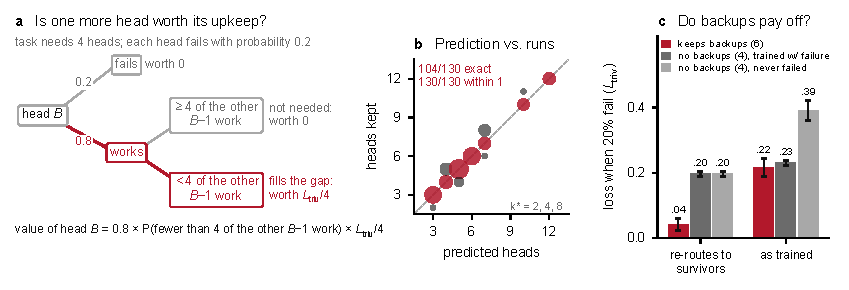
\includegraphics[width=\textwidth]{fig_backup_v2.pdf}
\caption{Redundancy under failure. \textbf{(a)} Each head fails with probability $p$. An extra head is worth something on one branch only: it works and fewer than $\kstar$ of the others do, so it supplies the missing answer, worth $\Ltriv/\kstar$. \textbf{(b)} Heads kept against the prediction in all 130 runs with failure ($\kstar=2,4,8$, $p$ from 0.05 to 0.3, two upkeeps). Dot size is the number of runs, red where exact. The first 30 runs came before the prediction was fixed, and the other 100 were predicted in writing before they started (79 exact, all within one head). \textbf{(c)} Loss when 20\% of the kept heads fail at test, 10 runs per arm, $\kstar=4$. With the read-out re-fitted to the survivors, the arm that kept backups loses five times less. As trained, training under failure gives most of the protection.}
\label{fig:backup}
\end{figure*}

\paragraph{A third prediction: redundancy under failure.} The objective also says how much redundancy to keep. Suppose each head fails independently with probability $p$ at every training step. An extra head then pays only when it works and fewer than $R$ of the others do (Figure~\ref{fig:backup}a), so the expected value of the $B$-th head is
\begin{equation}
v(B)=\frac{1-p}{R}\,\Pr\!\left[\mathrm{Bin}(B-1,1-p)<R\right]\Ltriv ,
\label{eq:backup}
\end{equation}
a $k$-out-of-$n$ calculation from reliability theory \citep{barlow1965reliability}, and the rule should keep the largest $B$ with $v(B)\ge\pi$. There is no free parameter. After 30 first runs, we committed predictions for 100 new runs before starting them, over $\kstar=2,4,8$, $p$ from 0.05 to 0.3 and two upkeeps. 79 matched exactly and all 100 were within one head (Figure~\ref{fig:backup}b). Two simpler guesses do far worse on the same runs: keeping $\kstar$ heads would match 4, and keeping enough heads that $\kstar$ work on average would match about 33. Most misses come from two settings that were off by one in every run.

To test whether the backups pay off, we trained three kinds of model for $\kstar=4$, 10 runs each: with failure and the rule (6 heads kept), with failure but with heads valued as if nothing failed (4 heads), and without failure (4 heads). When 20\% of the kept heads failed at test and the read-out was re-fitted to the survivors, the loss was $0.04\,\Ltriv$ with backups against $0.20$ without (Figure~\ref{fig:backup}c). Without the re-fit the gain is small, because training under failure already teaches the read-out to cope. This section tests the objective on a task where the right answer is known. We do not claim that backup heads in language models follow Equation~\eqref{eq:backup}.

\begin{figure}[t]
\centering
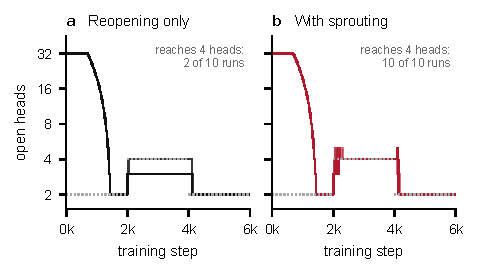
\includegraphics[width=\columnwidth]{fig_demand.pdf}
\caption{Changing demand: the number of needed heads goes from 2 to 4 and back to 2 (dotted), 10 runs each. \textbf{(a)} With reopening alone, the rule follows demand down but stalls at 3 heads on the way up in 8 of 10 runs. \textbf{(b)} With sprouting, it reaches 4 heads in every run.}
\label{fig:demand}
\end{figure}

\paragraph{Changing demand.} Vascular networks also grow where demand returns. We split training into three phases of 2000 steps in which 2, then 4, then 2 of four offsets are active. Two heads cannot solve the middle phase, since by Equation~\eqref{eq:law} their loss cannot fall below $0.5\,\Ltriv$. When demand fell, the rule closed back to exactly 2 heads in all 20 runs. When demand rose, reopening alone was not enough: 8 of 10 runs reopened one head and then stalled at 3 heads with a loss of $0.25\,\Ltriv$ for the whole phase (Figure~\ref{fig:demand}a). A closed head that never learned the new offset has no gain, so it never earns its reopening. With sprouting, 10 of 10 runs reached exactly 4 heads and solved the task in every phase (Figure~\ref{fig:demand}b). The regressed vessel and the closed head share a limitation, and the same remedy works for both.

\paragraph{Size.} With exactly $\kstar$ heads kept, deleting the closed heads leaves 6.3\%, 12.5\% and 25\% of the retrieval model's parameters for $\kstar=2,4,8$, and 30.3\% of the induction model's. During training the closed heads are still computed, so this saving is realized only once they are deleted.

\begin{figure*}[t]
\centering
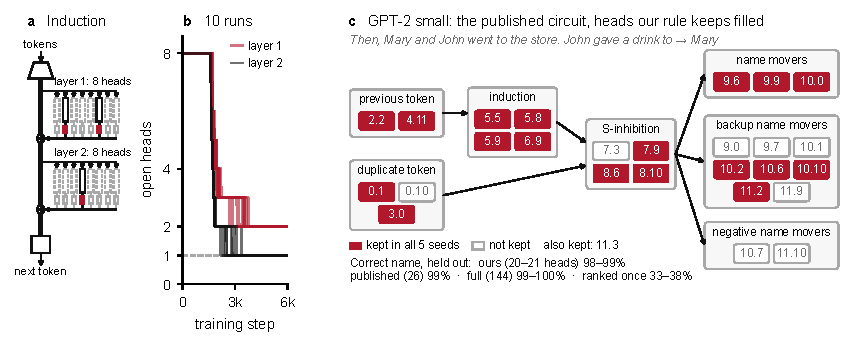
\includegraphics[width=\textwidth]{fig_circuits_v8.pdf}
\caption{Known circuits. \textbf{(a)} The induction model: two attention-only layers of 8 heads on a residual stream, each head with a valve. \textbf{(b)} Open heads per layer during training, 10 runs. Layer 2 closes to the one induction head. \textbf{(c)} GPT-2 small on indirect object identification, frozen weights, prompts of \citet{wang2023interpretability}. The 26 heads of the published circuit are grouped by the roles they assigned, from early to late layers, and a head (layer.head) is filled if our rule keeps it at the lowest upkeep in all 5 seeds. The rule assigns no roles. Bottom: held-out accuracy and logit difference (as \% of the full model), ranges over seeds. \emph{Ranked once}: the same number of heads, chosen by their single removal from the full model.}
\label{fig:circuits}
\end{figure*}

\section{Known Circuits}

\paragraph{Induction.} A two-layer attention-only model with $8+8$ heads, width 64 and a vocabulary of 64 tokens was trained for 6000 steps to continue a repeated sequence (Figure~\ref{fig:circuits}a). Its known circuit is a previous-token head in layer 1 and an induction head in layer 2 \citep{olsson2022}. The rule kept $2+1$ heads with the expected roles in 10 of 10 runs, and the task stayed solved (Figure~\ref{fig:circuits}b). Switching off the kept layer-2 head dropped accuracy on the repeat from 99.9\% to 1.8\%, chance for 64 tokens. The second layer-1 head acts as a backup: each layer-1 head alone missed about 1 in 8 repeated tokens, and together they missed about 1 in 200. Michel et al.\ lost the solution in all 10 runs.

\paragraph{GPT-2 small.} We applied the rule to the 144 heads of GPT-2 small on indirect object identification (Figure~\ref{fig:circuits}c), whose 26-head circuit was found by hand \citep{wang2023interpretability}. The weights were frozen, so this tests the valuing and re-valuing alone, without fade or reopening. Each of 5 seeds draws 300 prompts to choose heads and 1500 held-out prompts from the generator of \citet{wang2023interpretability}, which has 15 templates in both name orders. A closed head is replaced by its mean output on prompts with three different names, as in that work. The loss is the cross-entropy of the correct name, and the upkeep is a fraction (0.05, 0.02, 0.01) of the loss gap between all heads closed and all open.

At 1\% of the gap, the same scale as $0.01\,\Ltriv$ on the benchmark, where it kept the exact count in 9 of 9 runs, the rule kept 20--21 heads and picked the correct name in 98--99\% of held-out prompts, matching the published 26 heads (99.0--99.4\%) and the full model (99.1--99.8\%) with 5--6 fewer heads. They are the right heads: 19 of them are in the published circuit, 19 were kept in all 5 seeds, the name movers in all 15 runs, and the negative name movers, which push against the correct name, in none. Higher upkeeps gave nested subsets of 10--11 and 17--18 heads in every seed, so the upkeep trims the circuit rather than changing it (Table~\ref{tab:gpt2}). At the highest upkeep every kept head is in the published circuit.

\begin{table}[t]
\centering
\footnotesize
\setlength{\tabcolsep}{2.2pt}
\begin{tabular}{@{}lcccccc@{}}
\toprule
 & & \multicolumn{3}{c}{Correct name (\%)} & & \\
\cmidrule(lr){3-5}
Upkeep & Heads & Rule & \begin{tabular}[c]{@{}c@{}}Ranked\\once\end{tabular} & Random & \begin{tabular}[c]{@{}c@{}}In\\circuit\end{tabular} & \begin{tabular}[c]{@{}c@{}}Logit\\diff.\end{tabular} \\
\midrule
0.05 & 10--11 & 67--69 & 10--13 & 37--46 & 100\% & 26--29 \\
0.02 & 17--18 & 93--97 & 8--13 & 38--42 & 94\% & 90--109 \\
0.01 & 20--21 & 98--99 & 33--38 & 35--42 & 90--95\% & 121--124 \\
\midrule
Published & 26 & 99 & & & 100\% & 85--88 \\
Full model & 144 & 99--100 & & & & 100 \\
\bottomrule
\end{tabular}
\caption{GPT-2 small on indirect object identification, ranges over 5 seeds, 1500 held-out prompts each. \emph{Ranked once} and \emph{Random} use the same number of heads as the rule. \emph{In circuit}: share of the kept heads that are in the published circuit. \emph{Logit diff.}: correct-name logit minus subject logit for the rule's heads, as \% of the full model's.}
\label{tab:gpt2}
\end{table}

\paragraph{Re-valuing matters.} The same number of heads ranked once by their removal from the full model picked the correct name in only 33--38\% of prompts at 20--21 heads and 8--13\% at 17--18, below chance. Ranking once misses early heads whose value is hidden while their backups are present: each looks cheap to remove alone, but the later heads need at least one of them. On the logit difference, the measure of \citet{wang2023interpretability}, the rule's 20--21 heads recovered 121--124\% of the full model's, against 85--88\% for the published circuit, which is close to the 87\% they report. Exceeding the full model is consistent with closing the negative name movers.

\paragraph{A circuit, not a smaller model.} The kept heads are a circuit for one task, not a smaller general model. With only them open, a greater-than task fell to the level of random sets of the same size, and prediction of repeated tokens fell from 83\% to 18\%. Closing them alone left greater-than at 100\% but cut repeated tokens to 11--12\%, against 76--78\% when random sets of the same size were closed. The induction heads kept for this task are the ones repeated tokens rely on, an independent check that the rule finds mechanism and not a set of heads that merely fits the prompts.

\paragraph{Two further tasks.} At the middle upkeep, across 5 seeds, the rule kept 5 heads on greater-than and scored 97--100\%, against 93--97\% for the same number ranked once. On repeated tokens it kept 22--23 heads and scored 72--74\%, against 27--34\% for the same number ranked once and 84--85\% for the full model. Re-valuing helped in every seed on both tasks. The margin is small where a few late heads carry the task and large where the circuit has several steps with backups.

\section{Discussion}

Hemodynamic attenuation turns a principle of the cerebral circulation into a pruning rule with a stated cost. Like the vessels it is modeled on, it adapts the model's size to demand during training. Because the cost is explicit, what it does can be worked out in advance. The number of heads, the upkeep at which it collapses and the redundancy it keeps under failure each follow from the objective, and each was confirmed. In GPT-2 small, the same rule found a smaller, stable core of a circuit mapped by hand.

\paragraph{What each borrowed mechanism does.} Four properties come from the biology, and each was needed. The re-fit plays the role of collateral flow and removes copies. Gradual regression keeps the task solved while heads close. Reopening restores a head that becomes valuable. Sprouting is needed because a closed head, like a regressed vessel, cannot adapt until it is supplied again. Removing the first two broke the rule in the ablations, and removing the last broke it when demand rose.

\paragraph{What it predicts for the brain.} The correspondence in Figure~\ref{fig:hero} runs both ways. Equation~\eqref{eq:backup} would give the number of collateral vessels worth keeping from how often a vessel is occluded and what it costs to maintain: more where occlusion is likelier or tissue costlier to lose, none where upkeep exceeds the expected loss. That is a quantitative prediction about collateral supply that can be tested against vascular anatomy.

\paragraph{Limitations.} The models trained from scratch are small, so that their minimal circuits are known, and the retrieval model has a single layer. The re-fit is exact only for the output weights and a squared loss, and the induction and GPT-2 experiments use the simpler value without it. Proposition~1 covers fixed heads, while the fade, the warm-up and sprouting, which handle heads that are still learning, are justified empirically. The redundancy prediction was tested on the benchmark only. GPT-2 small was studied with frozen weights, so that experiment tests the value and the stopping rule but not pruning during training. Closed heads are still computed during training, so the compute saving comes only after they are deleted.

\paragraph{Next steps.} The natural test is the full rule, with fade and reopening, while a language model is being trained, where it can be compared with other pruning methods at equal size, and a head-to-head comparison with automated circuit discovery on GPT-2.

\bibliography{refs}

\end{document}
